%======================================================================
%===  dtuposter - a class to make posters tha comply with the DTU CI
%
% Written and maintained in 2011-2014 
% by Jorrit Wronski (jowr@mek.dtu.dk)
%
%
%==========================================
%===  details and poster setup
\documentclass[
%    ,title     = {{Title test}}
%    author    = {{Soeren Winkel Holm}}
%    ,subject   = {{This is the subject of my work}}
%    ,bgcolor   = dtulightgreen
%    ,highlight = dtuyellow
%    ,toplogo   = {{tex_dtu_aqua_b_uk}}
%    ,botlogo   = {{tex_dtu_bibliotek_b_uk}}
%    ,papersize = {{a0paper}}
%    ,colcount  = {{1column}}
%    ,longtitle
%    ,largecaption
%    ,draft
%    ,nocrop
%    ,english        % language
%    ,fleqn          % equations on the left
]{dtuposter}
%
%
%======================================================================
%===  Continue with packages
\usepackage[T1]{fontenc}        % special characters
%
%\usepackage[ansinew]{inputenc}  % Windows
%\usepackage[applemac]{inputenc} % MacOS
\usepackage[utf8]{inputenc}    % Unicode, Linux

%
% 
%======================================================================
%=== Font definitions, DTU recommends Arial for posters
%\usepackage{cmbright}
%\usepackage{arevmath}
%\usepackage[scaled]{uarial} %Arial clone, set as default sf font - use "ua1" for direct access
%\usepackage{uarial} %Arial clone, set as default sf font - use "ua1" for direct access
%\usepackage[typeface=default,
%            sanstypeface=urwarial,
%            mathtypeface=arevmath
%           ]{typeface}
\renewcommand{\familydefault}{\sfdefault}
\usepackage{enumitem}
\usepackage{amsmath}
\setlist{nosep,leftmargin=*}
%
% 
%======================================================================
%=== Other useful packages
\usepackage{booktabs}

\usepackage{float}
\usepackage[caption = false]{subfig}
%======================================================================
%=== The actual content starts here
\begin{document}
%
%
%======================================================================
%===  Make header for poster (title and authors)
\begin{dtuposterhead} %
\dtuposterauthor{Mads Andersen, Oskar Wiese, Anders Henriksen, Søren Holm, Asger Schultz}
\dtuposteraffil{DTU Compute}
\dtuposteraffil{\texttt{\{s173934, s183917, s183904, s183911, s183912\}@student.dtu.dk}}
\end{dtuposterhead}
%
%
%======================================================================
%===  ... and the rest of the content
\begin{dtupostercontent}
\section{Weeds, Crops and Dirt}

\begin{itemize}
	\item Motivation
	
	\item In this presentation
\end{itemize}
 
\section{The Data: Brazilian Sugar Fields}
The data used in this project is one drone image of a field, which is illustrated as the following.
\begin{figure}
\centering
\includegraphics[width=.7\linewidth]{raw-min}
\end{figure}


\section{Our SegNet: 1152 Feature Maps}

%%Model af netværket 
%%Encoder-Decoder
%% "Skip connections"" + Adam 

\begin{figure}
	\centering
	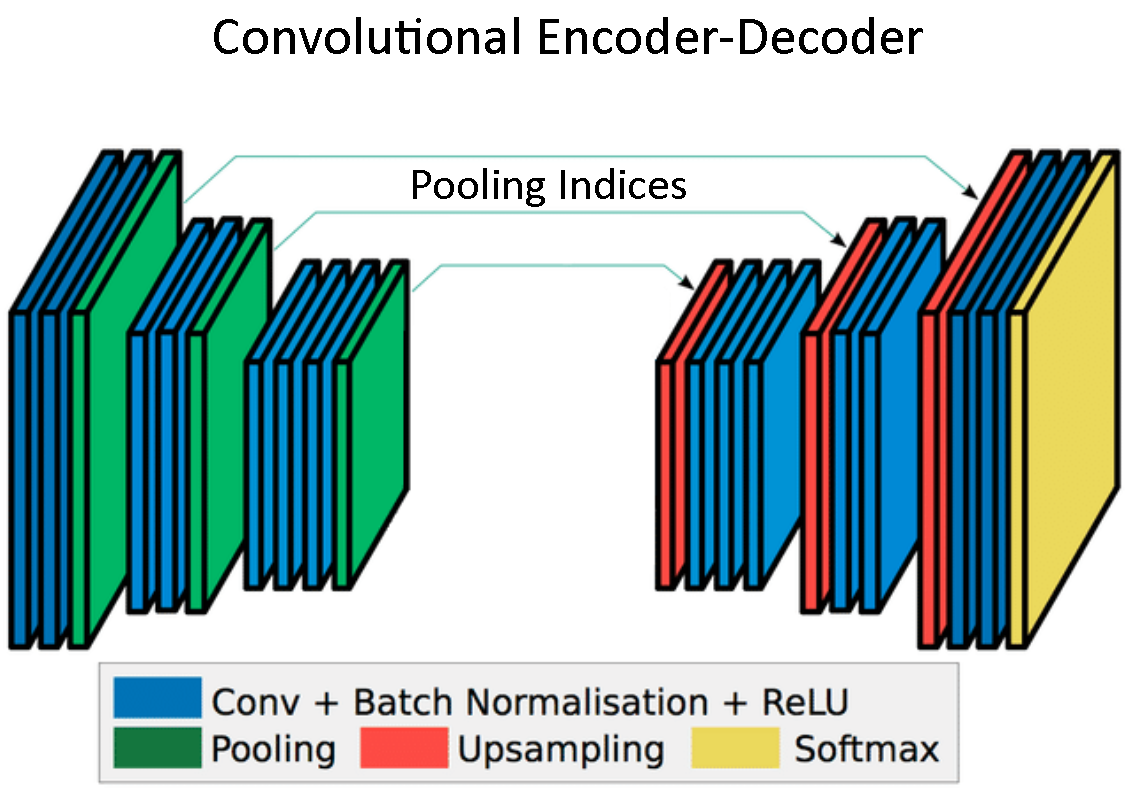
\includegraphics[width=0.8\linewidth]{Structure}
	\caption{}
	\label{fig:Structure}
\end{figure}
 
\begin{equation*}\label{key}
\scriptsize
\begin{bmatrix}a&b\\c&d\end{bmatrix} \xrightarrow{\text{\scriptsize M. pool indices}}
\begin{bmatrix}0&0&0&a\\b&0&0&0\\0&c&0&0\\0&0&d&0\end{bmatrix} 
\rightarrow 
\texttt{\scriptsize Conv2d}
\end{equation*}

The encoder part of the network creates a rich feature map representing the image content. The more 
layers of max-pooling there are the more translation invariance for robust 
classification can be achieved. The boundary detail is very important when 
dealing with image segmentation. Hence, capturing boundary information in 
the feature maps of the encoder before upsampling is important. This can 
simply be done by storing the whole feature map, but due to memory 
constrains only the maxpooling indices are saved, which is a good 
approximation of the feature maps. 


Loss of \(N\) pixels in one-hot \((N \times  3)\) matrix \(\mathbf x^pred\) with the true classes \(\mathbf c\).
\[
L = \frac 1 N \sum_{i=1}^{N} \mathbf{w}[i, c_i]  \cdot 
\left( 
-\mathbf x^\text{pred}[i, c_i] + \log
\left(
\sum_{j=1}^{3}\exp(\mathbf x^\text{pred}[i, j])
\right)
\right)
\]

\begin{itemize}
	\item Skip connections
	\item Max-pool
\end{itemize}


\begin{figure}
	\begin{fadebox}\begin{center}
			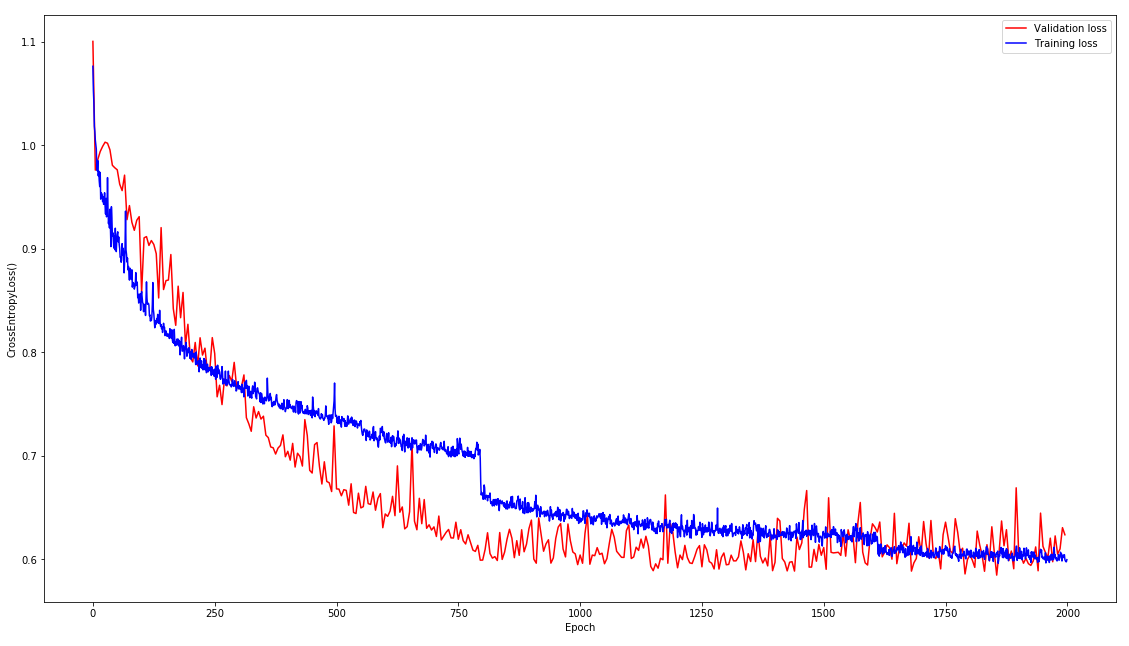
\includegraphics[width=\linewidth,origin=c]{loss}
	\end{center}\end{fadebox}
	\caption{An example caption. Figures can be wrapped in the \texttt{fadebox} 
		environment to provide them with a white background. Note that you have to align the 
		figure again.}\label{fig:example2}
\end{figure}

%% Hvordan regulariseres netværket
%% Data transformeringer 
%% Hyperparametre 

\section{Different Metrics, Different Stories}

%%Tabel med metrics 
%% Gøre vores F1 score fed og skriftstørrelse 100
\begin{table}
	\begin{tabular}{c|ccc|ccc|}
		
		\rule[-1ex]{0pt}{2.5ex}  & \multicolumn{3}{c|}{Train} &  \multicolumn{3}{c|}{Test} \\ 
		
		\rule[-1ex]{0pt}{2.5ex} Metric  & G & C & F1 & G & C & F1 \\ 
		\hline
		\rule[-1ex]{0pt}{2.5ex} Baseline&  33.3 &1.8  &3.4  &33.3  &1.1  &2.2  \\ 
		
		\rule[-1ex]{0pt}{2.5ex} U. SC. SegNet    &  &  &  &  &  &95.9  \\ 
		\rule[-1ex]{0pt}{2.5ex} U. SC. UNet   &  &  &  &  &  &92.9  \\ 
		\rule[-1ex]{0pt}{2.5ex} Cellari DNN   &  &  &  &  &  &77.7  \\ 
		\hline 
		\rule[-1ex]{0pt}{2.5ex} Our SegNet & 96.5&93.6  & 86.9 &97.5  & 90.7  &\textbf{84.6}  \\ 
	\end{tabular} 
\caption{Conclusions lala note cellari has not provided more scores note U. SC. does not have same test set}
\end{table}



%Kort beskrivelse af resultater 

\begin{figure}
	\centering
\subfloat{
	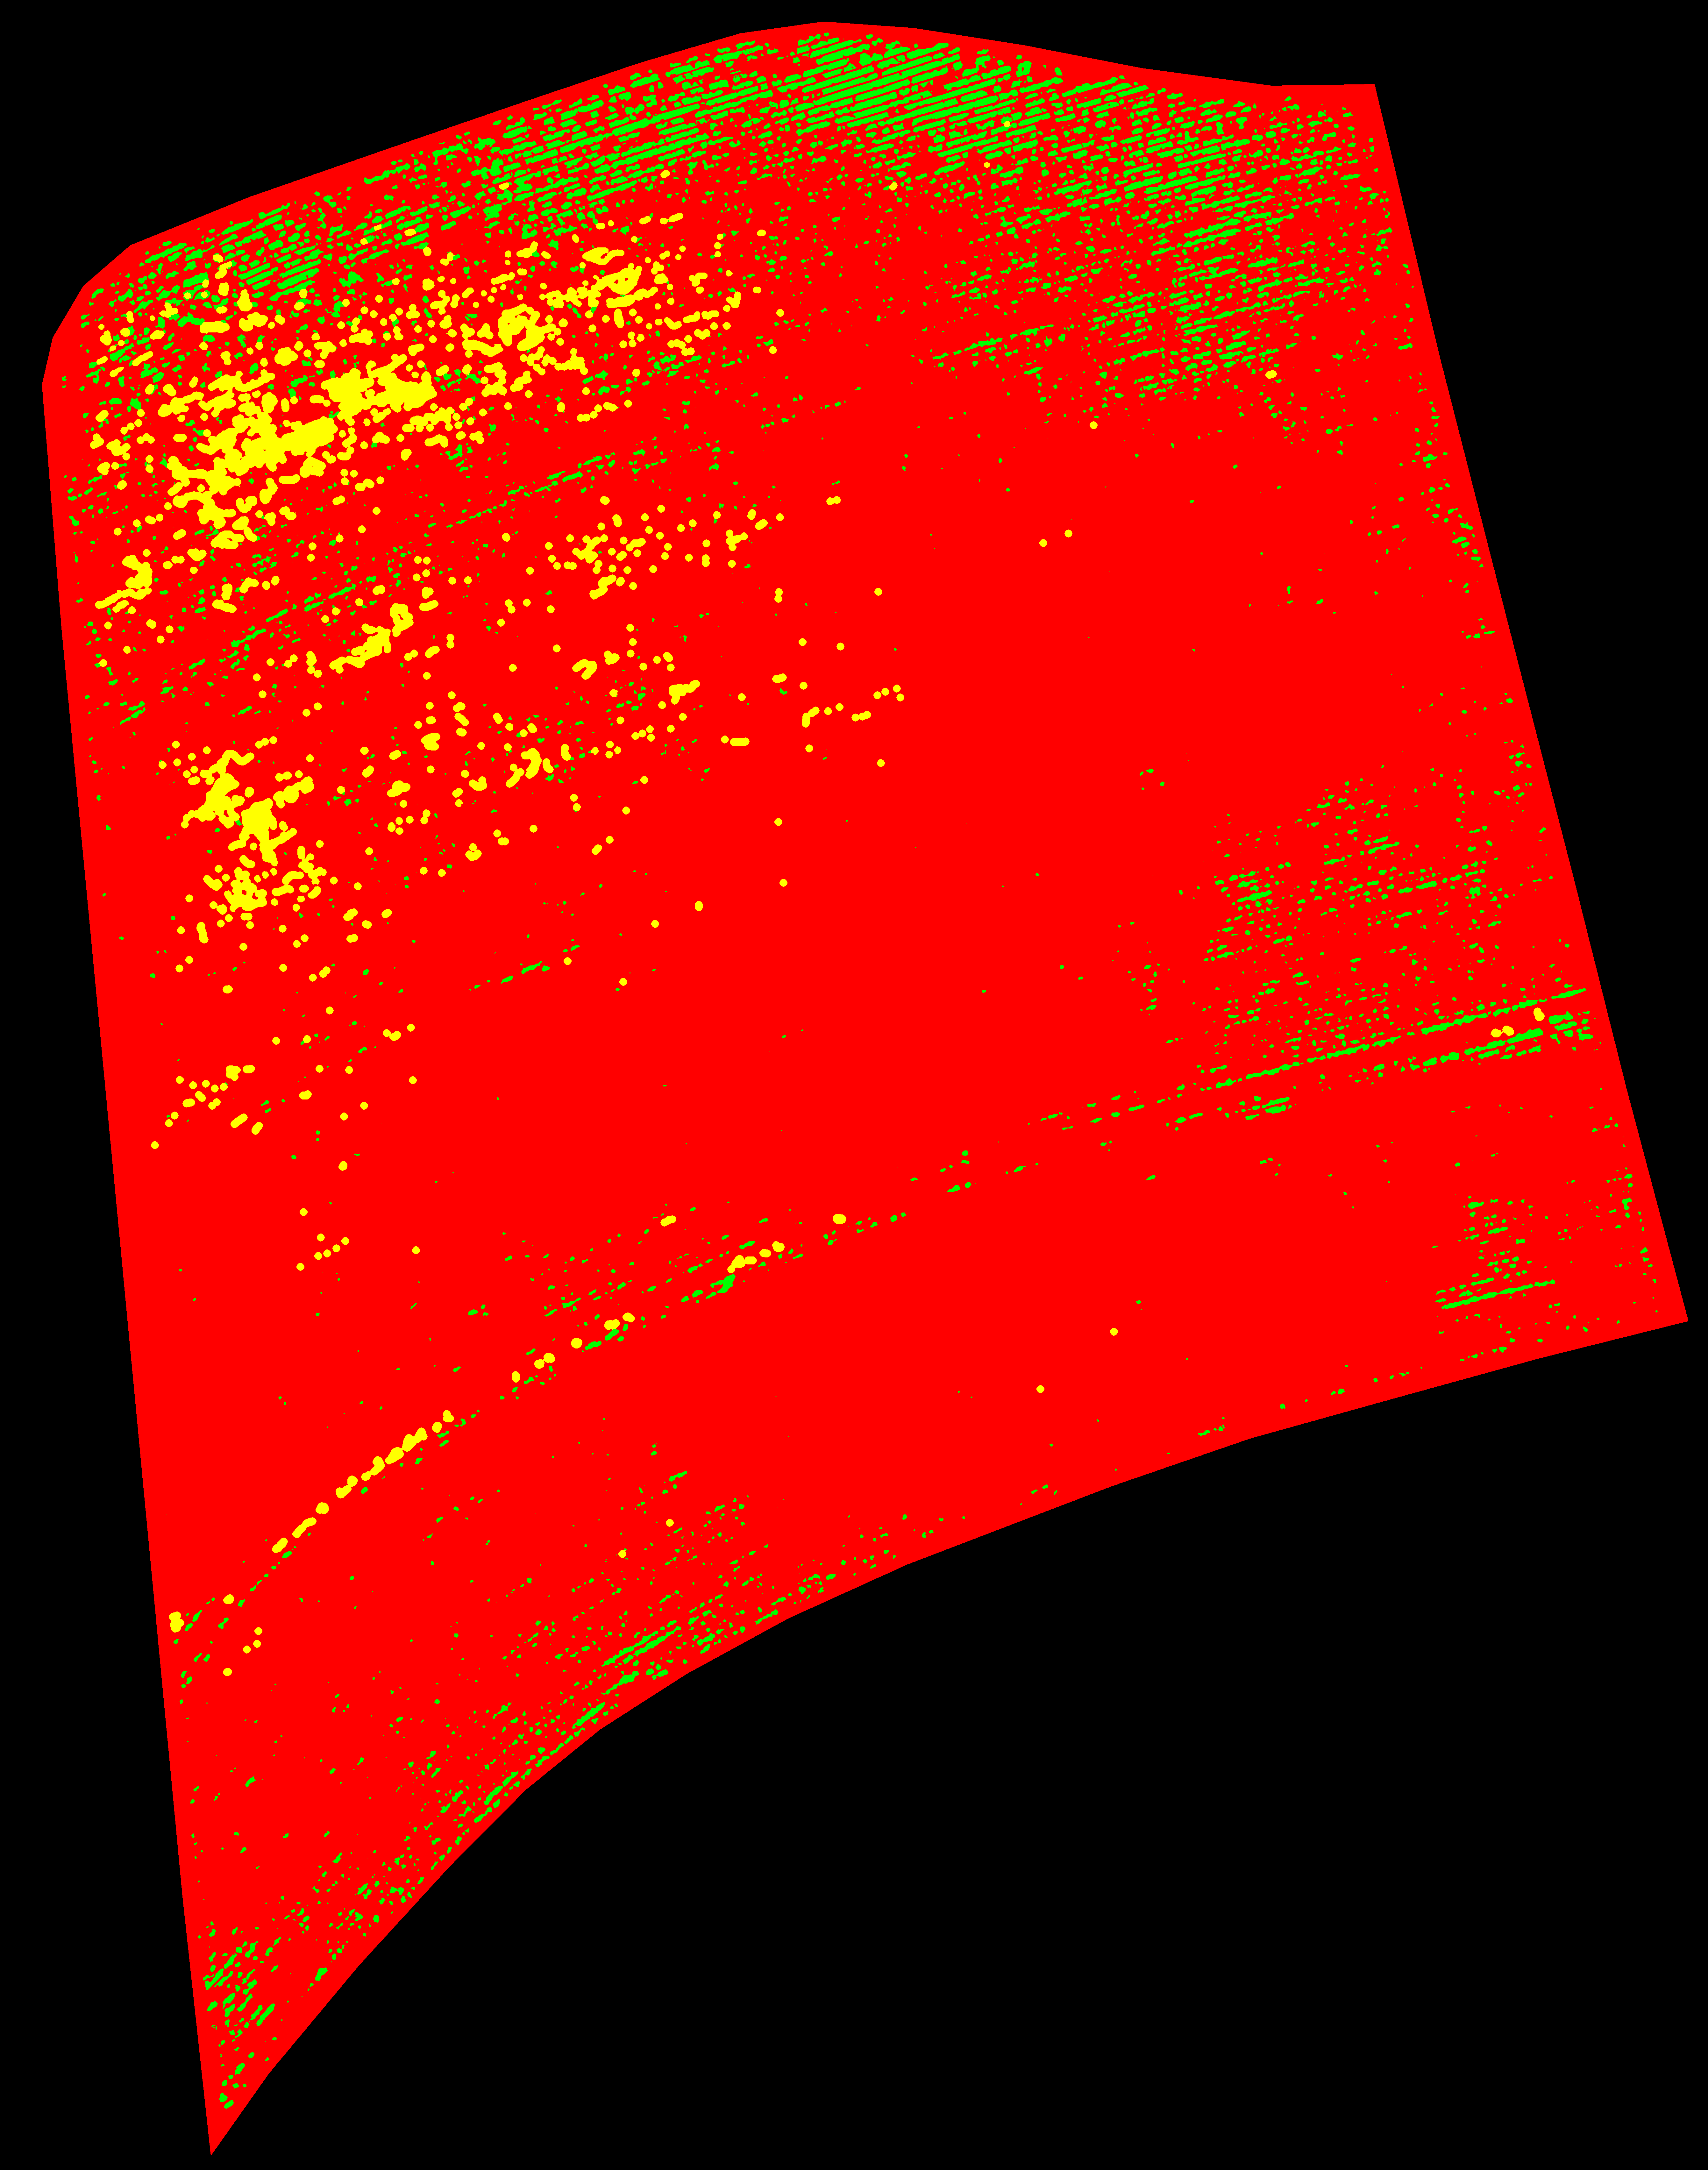
\includegraphics[width=.5\linewidth]{target}	
}
\subfloat{
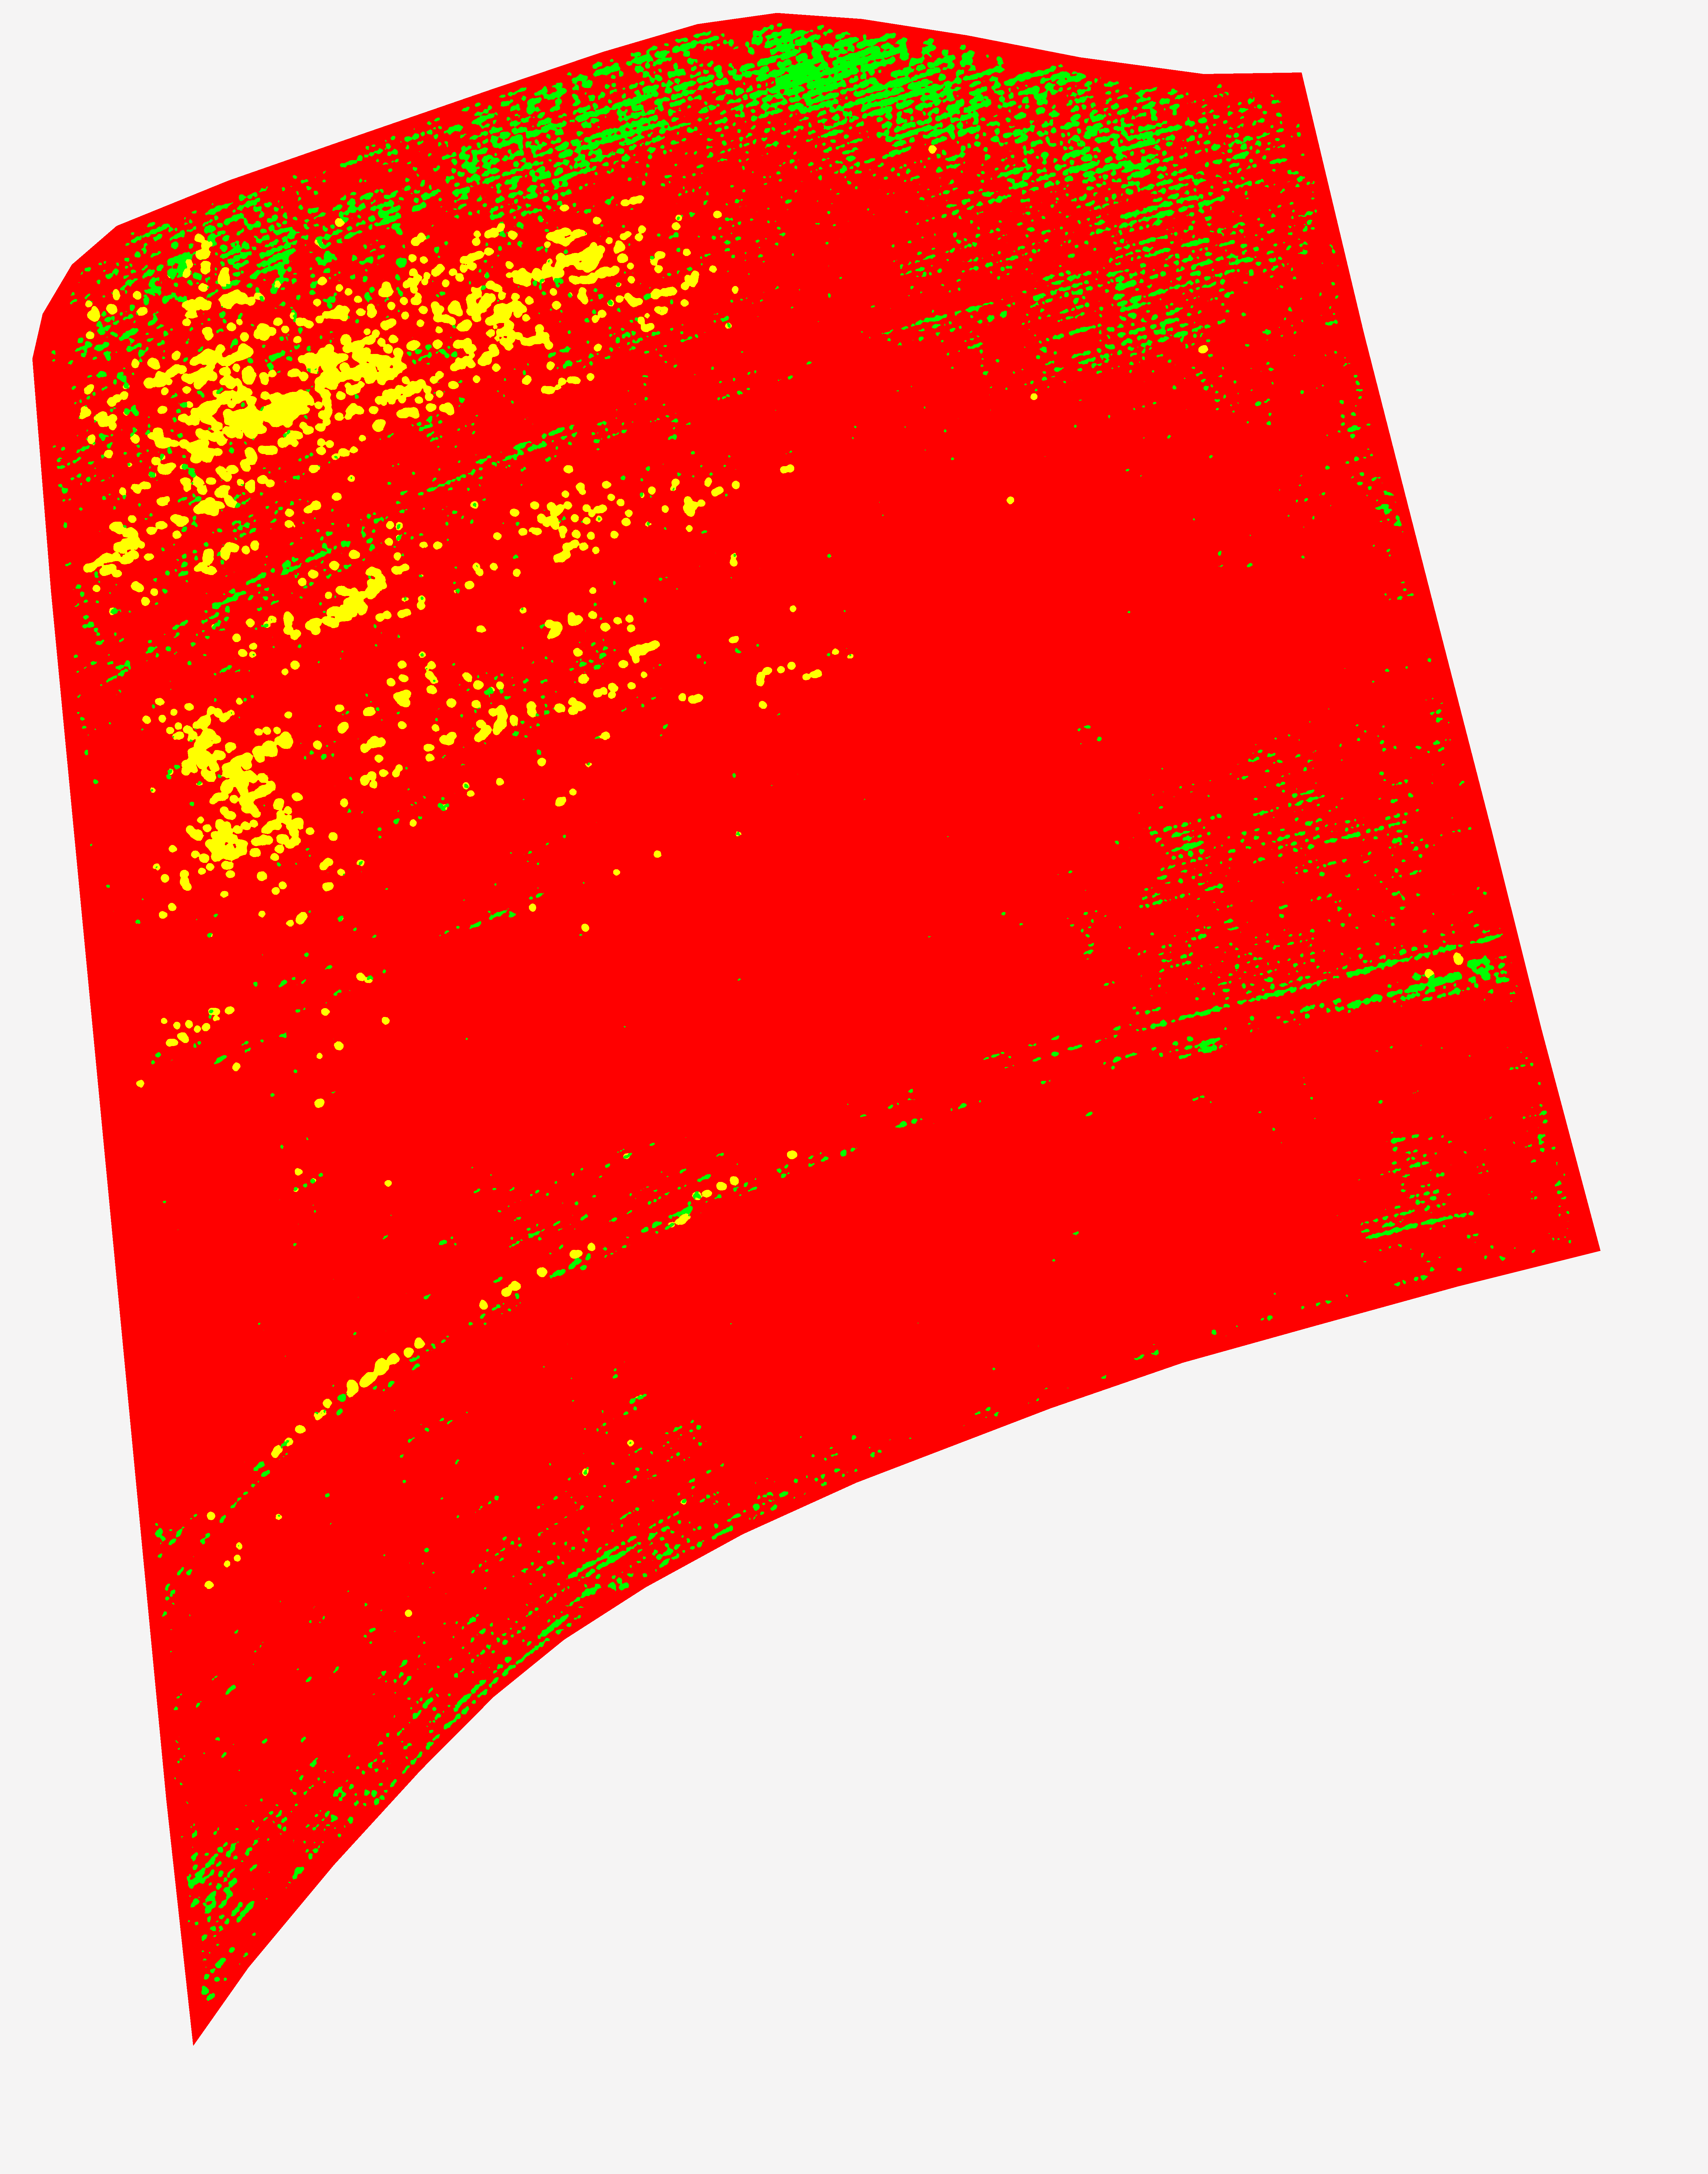
\includegraphics[width=.5\linewidth]{anno}	
}
\caption{An example caption. This figure supports transparency and looks fine on 
the coloured background}\label{fig:example}
\end{figure}


\section{Where Can This Go?}
% Yderligere arbejde
%Perspektiv på problemet 

\begin{figure}
	\begin{fadebox}\begin{center}
			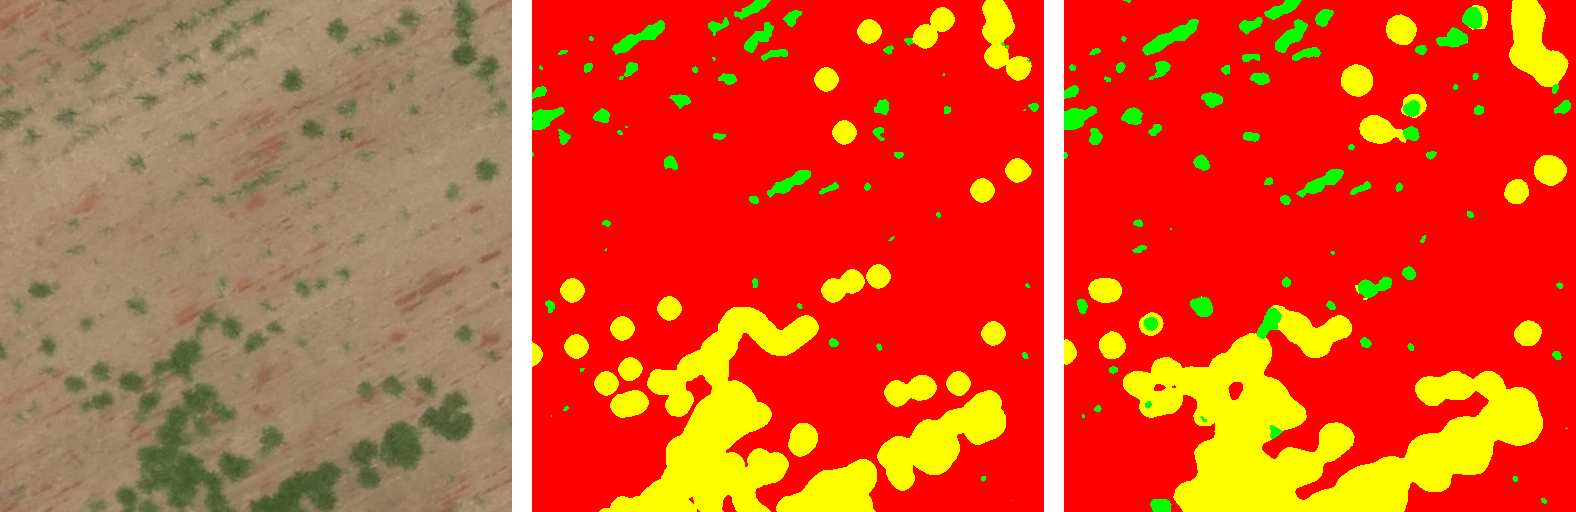
\includegraphics[width=\linewidth,origin=c]{reconst}
	\end{center}\end{fadebox}
\end{figure}


\end{dtupostercontent}
\end{document}
